\documentclass[whitelogo]{tudelft-report}
\usepackage{graphicx}
\usepackage{subcaption}
\usepackage{gensymb}
\usepackage{changes}
\begin{document}
%% Use Roman numerals for the page numbers of the title pages and table of
%% contents.
\frontmatter


%% Uncomment following 16 lines for a cover with a picture on the lower half only
\title[tudelft-white]{Assignment 1}
\subtitle[tudelft-black]{GEO1001}
\author[tudelft-white]{Louise Spekking}
\affiliation{Technische Universiteit Delft}
\coverimage{Assignment_1.png}
\covertext[tudelft-white]{
    \textbf{4256778} \\
     \\
       \vfill
}
\setpagecolor{tudelft-cyan}
\makecover[split]


%% Include an optional title page.
%\input{title}

%\input{preface}

\tableofcontents


%% Use Arabic numerals for the page numbers of the chapters.
\mainmatter



\section {A1}
As the first assignment the mean, the variance and the standard deviation of all 19 numeric variables were calculated, for report clarity these tables are not displayed here, but are uploaded as ckv files to GitHub. 
\\
In figure \ref{fig:hist5and50} two histograms of the temperature measurements are shown. When comparing the two histograms the importance of the number of bins can be ….?? Details about the distribution of the data points are visible in the histogram with 50 bins, however in the histogram with 5 bins many nuances of the distribution are lost. 
 


\begin{figure}[h!]
  \centering
  \begin{subfigure}[b]{0.4\linewidth}
    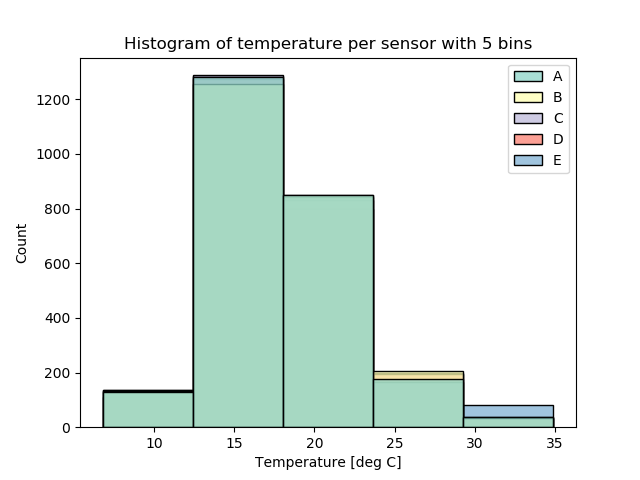
\includegraphics[width=\linewidth]{Histogram of temperature per sensor with 5 bins.png}
    \caption{Coffee.}
  \end{subfigure}
  \begin{subfigure}[b]{0.4\linewidth}
    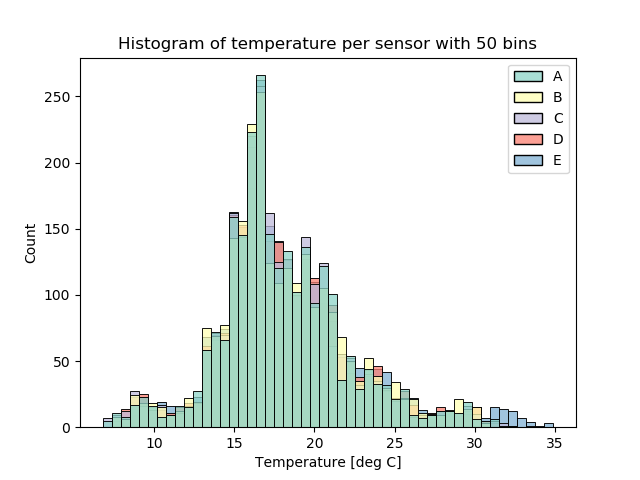
\includegraphics[width=\linewidth]{Histogram of temperature per sensor with 50 bins.png}
    \caption{More coffee.}
  \end{subfigure}
  \caption{Histograms of the temperature measured by all 5 sensors in \degree C, with 5 and 50 bins.}
  \label{fig:hist5and50}
\end{figure}


\begin{figure}[h!]
  \centering
  \begin{subfigure}[b]{0.4\linewidth}
    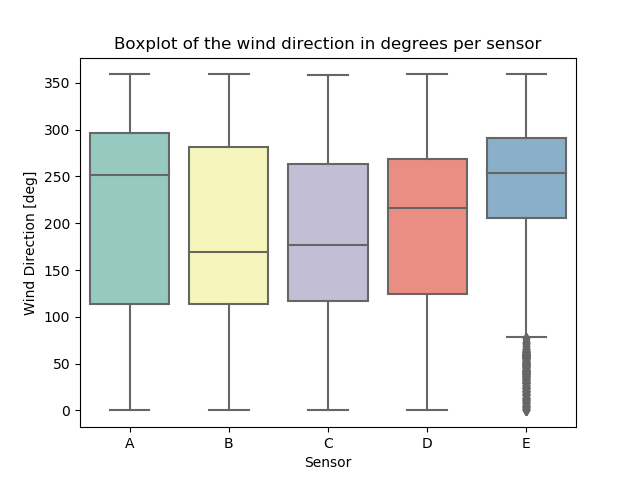
\includegraphics[width=\linewidth]{Boxplot of the wind direction in degrees per sensor.png}
    \caption{Boxplot of wind direction per sensor}
  \end{subfigure}
  \begin{subfigure}[b]{0.4\linewidth}
    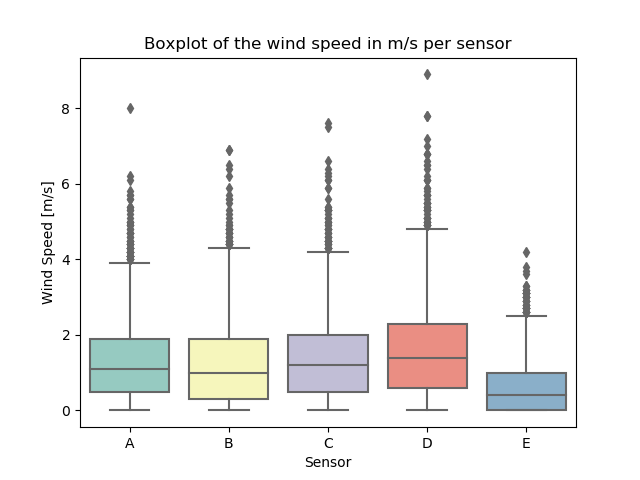
\includegraphics[width=\linewidth]{Boxplot of wind speed.png}
    \caption{Boxplot of wind speed per sensor}
  \end{subfigure}
  \begin{subfigure}[b]{0.4\linewidth}
    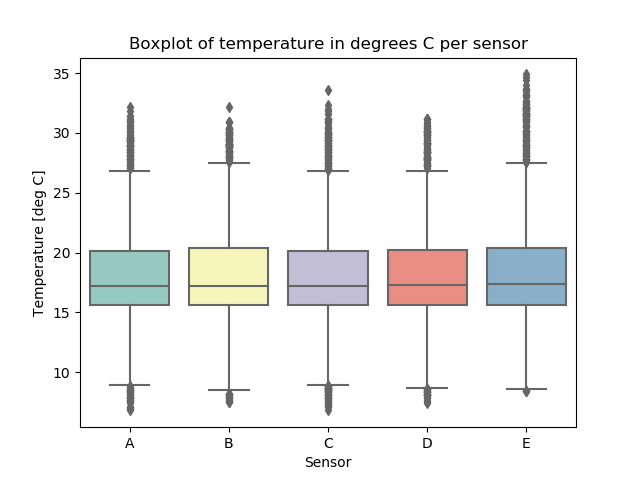
\includegraphics[width=\linewidth]{Boxplot of temperature per sensor.png}
    \caption{Boxplot of temperature per sensor}
  \end{subfigure}
  \caption{Boxplots showing the data for wins direction wind speed and temperature for all 5 sensors}
  \label{fig:boxplots}
\end{figure}





\section {A2}


\section {A3}


%\input{chapter-1}

%% Use letters for the chapter numbers of the appendices.
\appendix

%\input{appendix-a}

\bibliography{report}

\end{document}

